\documentclass[crop=true, border=10pt]{standalone}
\usepackage{amsmath}

\usepackage{xcolor}

\usepackage{tikz}
\usetikzlibrary{arrows.meta}
\usetikzlibrary{decorations.markings}

\usepackage{tikz-3dplot}

\usepackage{pgfplots}

\usepackage{colortbl}

% A few colors
%--------------------------------------------------------------
\definecolor{plum}{rgb}{0.36078, 0.20784, 0.4}
\definecolor{chameleon}{rgb}{0.30588, 0.60392, 0.023529}
\definecolor{cornflower}{rgb}{0.12549, 0.29020, 0.52941}
\definecolor{scarlet}{rgb}{0.8, 0, 0}
\definecolor{brick}{rgb}{0.64314, 0, 0}
\definecolor{sunrise}{rgb}{0.80784, 0.36078, 0}
\definecolor{lightblue}{rgb}{0.15,0.35,0.75}



\begin{document}


\pagestyle{empty}

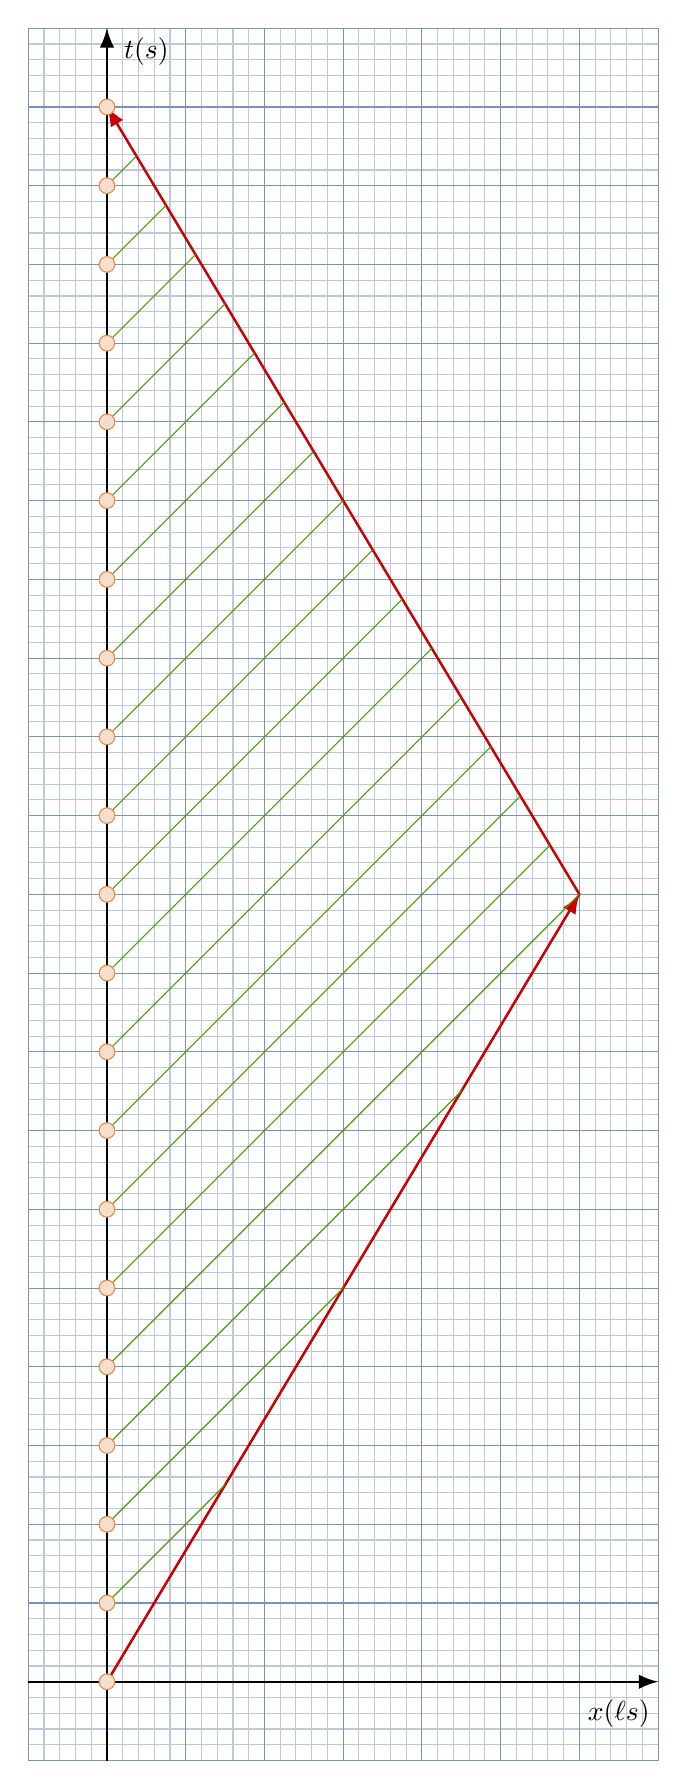
\begin{tikzpicture}[scale=1,domain=0:6]
	\tikzstyle{axisarrow} = [-{Latex[inset=0pt,length=7pt]}]

	% Draw the grid.
	\draw [cornflower!30,step=0.2,thin] (-1,-1) grid (7,21);
	\draw [cornflower!60,step=1.0,thin] (-1,-1) grid (7,21);

	% Clip all lines that would fall outside the grid
	\clip(-1,-1) rectangle (7,21);
	
	% Draw Axes
	\draw[thick,axisarrow] (0,-1) -- (0,21);
	\node[inner sep=0pt] at (0.5,20.7) {$t (s)$};
	\draw[thick,axisarrow] (-1,0) -- (7,0);
	\node[inner sep=0pt] at (6.5,-0.4) {$x (\ell s)$};

	
	
	\draw[scarlet,thick,axisarrow] (0,0) -- (3*10/5,10);
	\draw[scarlet,thick] plot (\x,5*\x/3);

	\draw[scarlet,thick,axisarrow] (6,10) -- (0,20);
	\draw[scarlet,thick] plot (\x,-5*\x/3+20);


	\begin{scope}
		\clip (0,0) -- (6,10) -- (0,20) -- (0,0);

		\foreach \t in {0,1,2,...,20}
		{
			\draw[chameleon] (0,1*\t) -- (7,7 + \t);
		}    	
				
	\end{scope}


    	\foreach \t in {0,1,...,20}
		{
			\node at (0,1*\t) [circle,draw=sunrise!70,fill=sunrise!20,inner sep=2pt] {};
		}	

\end{tikzpicture}			
\hskip1em
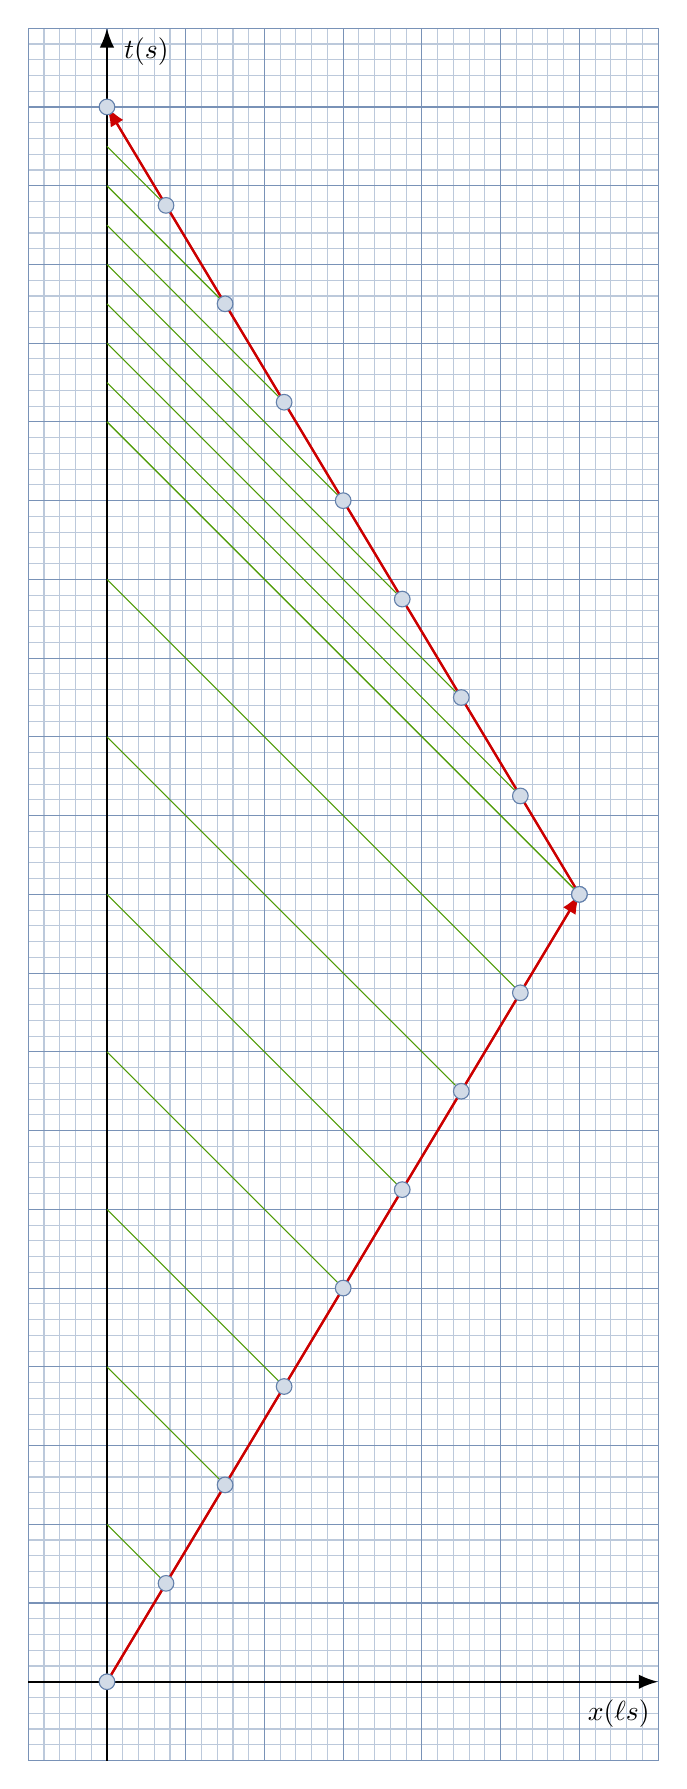
\begin{tikzpicture}[scale=1,domain=0:6]
	\tikzstyle{axisarrow} = [-{Latex[inset=0pt,length=7pt]}]

	% Draw the grid.
	\draw [cornflower!30,step=0.2,thin] (-1,-1) grid (7,21);
	\draw [cornflower!60,step=1.0,thin] (-1,-1) grid (7,21);

	% Clip all lines that would fall outside the grid
	\clip(-1,-1) rectangle (7,21);
	
	% Draw Axes
	\draw[thick,axisarrow] (0,-1) -- (0,21);
	\node[inner sep=0pt] at (0.5,20.7) {$t (s)$};
	\draw[thick,axisarrow] (-1,0) -- (7,0);
	\node[inner sep=0pt] at (6.5,-0.4) {$x (\ell s)$};

	
	\draw[scarlet,thick,axisarrow] (0,0) -- (3*10/5,10);
	\draw[scarlet,thick] plot (\x,5*\x/3);

	\draw[scarlet,thick,axisarrow] (6,10) -- (0,20);
	\draw[scarlet,thick] plot (\x,-5*\x/3+20);


	\begin{scope}
		\clip (0,0) -- (6,10) -- (0,20) -- (0,0);
    	
				
	\end{scope}

		\foreach \tp in {0,1,2,...,8}
		{
			\draw[chameleon] (0.75*\tp,1.25*\tp) -- (0,2*\tp);
		}
		\foreach \tp in {0,1,2,...,8}
		{
			\draw[chameleon] (6-0.75*\tp,10+1.25*\tp) -- (0,16+0.5*\tp);
		}

    	\foreach \tp in {0,1,...,8}
		{
			\node at (0.75*\tp,1.25*\tp) [circle,draw=cornflower!70,fill=cornflower!20,inner sep=2pt] {};
		}	

	    \foreach \tp in {0,1,...,8}
		{
			\node at (6-0.75*\tp,10+1.25*\tp) [circle,draw=cornflower!70,fill=cornflower!20,inner sep=2pt] {};
		}

\end{tikzpicture}
\hskip1em
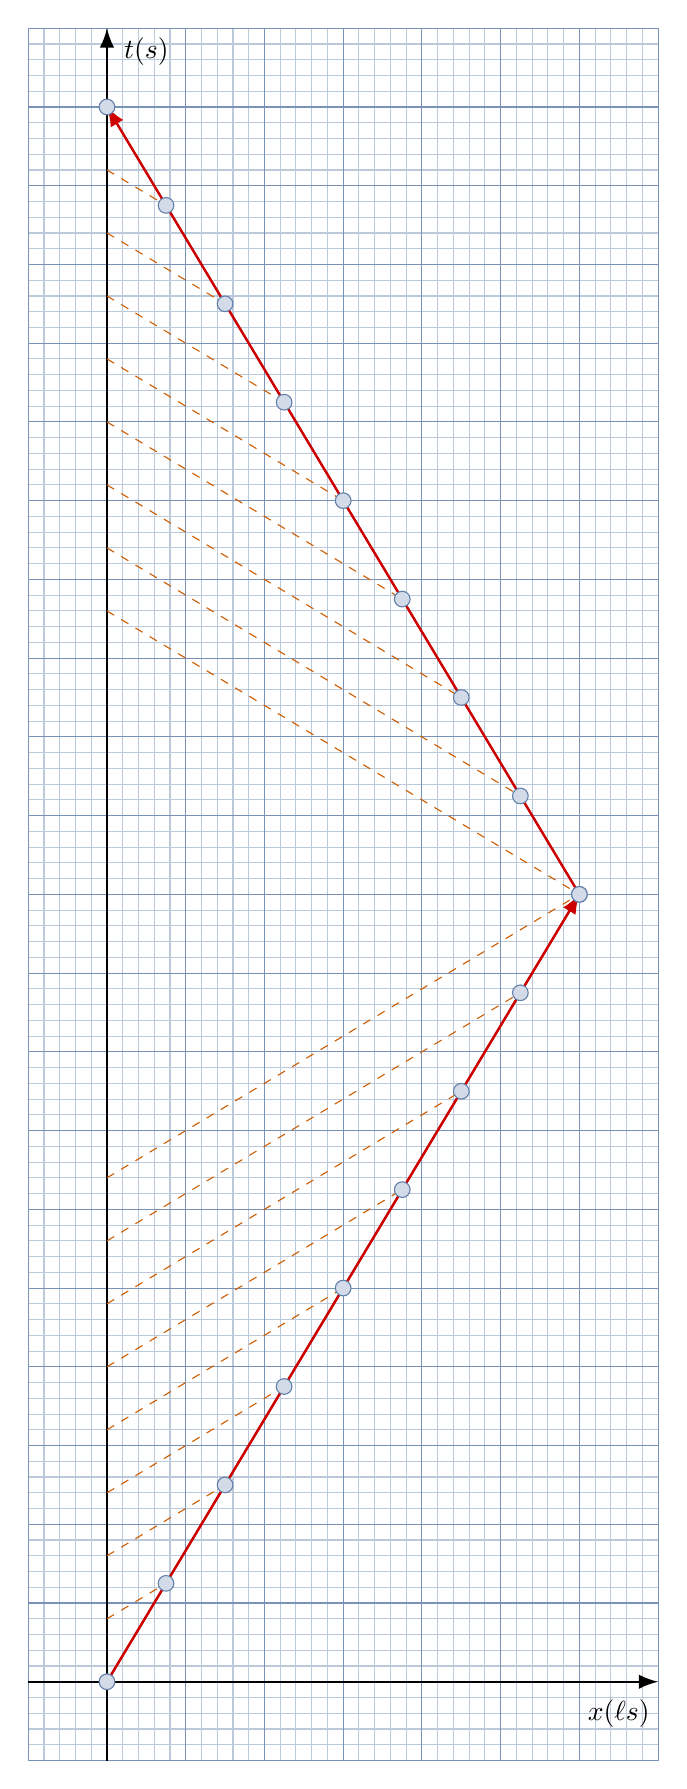
\begin{tikzpicture}[scale=1,domain=0:6]
	\tikzstyle{axisarrow} = [-{Latex[inset=0pt,length=7pt]}]

	% Draw the grid.
	\draw [cornflower!30,step=0.2,thin] (-1,-1) grid (7,21);
	\draw [cornflower!60,step=1.0,thin] (-1,-1) grid (7,21);

	% Clip all lines that would fall outside the grid
	\clip(-1,-1) rectangle (7,21);
	
	% Draw Axes
	\draw[thick,axisarrow] (0,-1) -- (0,21);
	\node[inner sep=0pt] at (0.5,20.7) {$t (s)$};
	\draw[thick,axisarrow] (-1,0) -- (7,0);
	\node[inner sep=0pt] at (6.5,-0.4) {$x (\ell s)$};

	
	
	\draw[scarlet,thick,axisarrow] (0,0) -- (3*10/5,10);
	\draw[scarlet,thick] plot (\x,5*\x/3);

	\draw[scarlet,thick,axisarrow] (6,10) -- (0,20);
	\draw[scarlet,thick] plot (\x,-5*\x/3+20);


	\begin{scope}
		\clip (0,0) -- (6,10) -- (0,20) -- (0,0);
    	
		\foreach \tp in {0,1,2,...,8}
		{
			\draw[dashed, sunrise] plot (\x,0.6*\x + 0.8*\tp);
		}
		
    	\foreach \tp in {0,1,2,...,8}
		{
			\draw[dashed, sunrise] plot (\x,-0.6*\x + 0.8*\tp+ 13.6);
		}
				
	\end{scope}

    	\foreach \tp in {0,1,...,8}
		{
			\node at (0.75*\tp,1.25*\tp) [circle,draw=cornflower!70,fill=cornflower!20,inner sep=2pt] {};
			}	

	    \foreach \tp in {0,1,...,8}
		{
			\node at (6-0.75*\tp,10+1.25*\tp) [circle,draw=cornflower!70,fill=cornflower!20,inner sep=2pt] {};
		}

\end{tikzpicture}		
\end{document}